\PassOptionsToPackage{unicode}{hyperref}
\PassOptionsToPackage{hyphens}{url}
%
\documentclass[11pt]{article}

\usepackage[top=1in, bottom=1in, left=1in, right=1in]{geometry}
\usepackage{amsmath}
\usepackage{enumerate}
\usepackage{tabularx}
\usepackage{graphicx}
\usepackage{iftex}
\ifPDFTeX
  \usepackage[T1]{fontenc}
  \usepackage[utf8]{inputenc}
  \usepackage{textcomp}
\else
  \usepackage{unicode-math}
  \defaultfontfeatures{Scale=MatchLowercase}
  \defaultfontfeatures[\rmfamily]{Ligatures=TeX,Scale=1}
\fi
\usepackage{lmodern}
\ifPDFTeX\else
  \setmathfont{Latin Modern Math}
  \newfontfamily\unicodefont{DejaVu Sans Mono}[Scale=0.85]
  \ifLuaTeX
    \usepackage{luatexja-fontspec}
    \setmainjfont{Noto Sans CJK SC}[Scale=0.9]
  \else
    \usepackage{xeCJK}
    \setCJKmainfont{Noto Sans CJK SC}[Scale=0.9]
  \fi
  \newcommand{\cjkfont}{}
\fi
\IfFileExists{upquote.sty}{\usepackage{upquote}}{}
\IfFileExists{microtype.sty}{%
  \usepackage[]{microtype}
  \UseMicrotypeSet[protrusion]{basicmath}
}{}
\makeatletter
\@ifundefined{KOMAClassName}{%
  \IfFileExists{parskip.sty}{%
    \usepackage{parskip}
  }{%
    \setlength{\parindent}{0pt}
    \setlength{\parskip}{6pt plus 2pt minus 1pt}}
}{%
  \KOMAoptions{parskip=half}}
\makeatother
\usepackage{xcolor}
\usepackage{tikz}
\usetikzlibrary{arrows.meta,calc,decorations.pathreplacing}

\definecolor{ccL1}{HTML}{dce8f5}
\definecolor{ccL1e}{HTML}{aec8e0}
\definecolor{ccL1b}{HTML}{7aacc8}
\definecolor{ccL2}{HTML}{c6dbef}
\definecolor{ccL2e}{HTML}{91bdd6}
\definecolor{ccL2b}{HTML}{5a8fb0}
\definecolor{ccL3}{HTML}{3182bd}
\definecolor{ccL3e}{HTML}{1a5f99}
\definecolor{ccL4}{HTML}{08519c}
\definecolor{ccL4e}{HTML}{06346a}
\definecolor{ccGap}{HTML}{cc2222}
\definecolor{ccRed}{HTML}{cc2222}
\definecolor{ccBlu}{HTML}{2266cc}
\definecolor{ccPur}{HTML}{7b2d8e}
\definecolor{ccSeam}{HTML}{d4a017}

\usepackage{longtable,booktabs,array}
\newcolumntype{Y}{>{\raggedright\arraybackslash}X}
\newcolumntype{P}[1]{>{\raggedright\arraybackslash}p{#1}}
\usepackage{calc}
\usepackage{etoolbox}
\makeatletter
\patchcmd\longtable{\par}{\if@noskipsec\mbox{}\fi\par}{}{}
\makeatother
\IfFileExists{footnotehyper.sty}{\usepackage{footnotehyper}}{\usepackage{footnote}}
\makesavenoteenv{longtable}
\setlength{\emergencystretch}{3em}
\providecommand{\tightlist}{%
  \setlength{\itemsep}{0pt}\setlength{\parskip}{0pt}}
\setcounter{secnumdepth}{3}
\newlength{\cslhangindent}
\setlength{\cslhangindent}{1.5em}
\newlength{\csllabelwidth}
\setlength{\csllabelwidth}{3em}
\newlength{\cslentryspacingunit}
\setlength{\cslentryspacingunit}{\parskip}
\newenvironment{CSLReferences}[2]
 {%
  \setlength{\parindent}{0pt}
  \ifodd #1
  \let\oldpar\par
  \def\par{\hangindent=\cslhangindent\oldpar}
  \fi
  \setlength{\parskip}{#2\cslentryspacingunit}
 }%
 {}
\newcommand{\CSLBlock}[1]{#1\hfill\break}
\newcommand{\CSLLeftMargin}[1]{\parbox[t]{\csllabelwidth}{#1}}
\newcommand{\CSLRightInline}[1]{\parbox[t]{\linewidth - \csllabelwidth}{#1}\break}
\newcommand{\CSLIndent}[1]{\hspace{\cslhangindent}#1}
\ifLuaTeX
  \usepackage{selnolig}
\fi
\IfFileExists{bookmark.sty}{\usepackage{bookmark}}{\usepackage{hyperref}}
\IfFileExists{xurl.sty}{\usepackage{xurl}}{}
\urlstyle{same}
\hypersetup{
  hidelinks,
  pdfcreator={LaTeX via pandoc}}

\renewcommand{\topfraction}{0.9}
\renewcommand{\bottomfraction}{0.8}
\renewcommand{\textfraction}{0.1}
\renewcommand{\floatpagefraction}{0.8}

\usepackage{natbib}

\title{The Constraint Cascade: A Diagnostic Taxonomy for AI Governance Failure}
\author{Lucia Yizi Zhang\\Shanghai Lixin University of Accounting and Finance}
\date{}

\begin{document}

\begin{abstract}
AI governance lacks a diagnostic vocabulary for locating failure within the deployment architecture. When a language-model agent produces harm, existing frameworks ask whether the model or the user is at fault---a binary that collapses four structurally distinct layers of constraint into an uninformative dyad. We introduce the Constraint Cascade, a four-layer diagnostic taxonomy that partitions LLM deployment into Environment (L1), Interface (L2), Algorithm \& Weights (L3), and Strategic Authority (L4). Between L2 and L3 lies an \emph{epistemic boundary}: we take as a premise, established in companion work~\cite{anon2026dual}, that an agent's operative state can be provably non-recoverable from its visible trace while remaining relevant to the next action. Read through systems safety, this is a defect Leveson's STPA cannot reach---the feedback a controller needs to keep a correct process model is here capacity-bounded by construction, not contingently broken. We therefore recast the four layers as a hierarchical control structure in which the Interface (L2) is a \emph{platform controller} acting on the model (L3) across that boundary; the human ``friction-seam'' labor (moderators, alignment researchers) are the controllers stationed on the bounded feedback path, absorbing misalignment cost along strict power gradients without the observational authority to close it. From this structure we derive the Unsafe Control Actions the architecture admits and map three loss-scenario classes---Override, Contamination, and Compression---to the positions where the control loop fractures, illustrated across four real-world cases ranging from no human agency to full deployer intent. The Cascade provides governance institutions with a structural vocabulary for diagnostic auditing, separating the question of \textit{which layer failed} from the downstream legal question of \textit{who bears responsibility}.
\end{abstract}

\maketitle

% ============================================================
\section{Introduction}
% ============================================================

In October 2018, Lion Air Flight 610 crashed thirteen minutes after takeoff, killing 189 people. Five months later, Ethiopian Airlines Flight 302 followed the same trajectory, killing 157 more. Investigations revealed that Boeing's Maneuvering Characteristics Augmentation System (MCAS) relied on a single angle-of-attack sensor; when that sensor produced erroneous readings, MCAS repeatedly overrode pilot control inputs to push the nose down. The failure was not in the sensor, the software, or the pilots individually---it was in the interaction between layers of a constraint architecture that no single actor fully understood or controlled~\cite{jatr2019737max}.

AI system safety faces an analogous diagnostic problem in a more acute form. Multiple control nodes---users, interfaces, alignment algorithms, corporate roadmaps---shape system behavior through hierarchical control loops at different architectural layers. When these control signals conflict or feedback loops fracture, the resulting emergent hazards are not attributable to any individual component, and existing alignment paradigms lack the cybernetic vocabulary to identify where the control loop broke, which actuator was saturated, and where architectural redundancy should concentrate.

But the analogy breaks at a critical point. Systems-theoretic accident models like Leveson's STPA~\cite{leveson2012engineering, leveson2018stpa} locate causation in control-structure failures across hierarchical layers, presupposing that safe states are physically defined facts---correct airspeed, proper control-surface deflection, intact structural load paths. AI deployment lacks this property at the operational level. Terminal outcomes---death, injury, military targeting---may be uncontested, but the operational safe states that precede them (what counts as crisis-detection threshold, what counts as legitimate military use, what counts as acceptable training-data norms) are contested, layer-dependent, and retrospectively constructed. STPA decomposes safety into well-defined sub-states at each hierarchical level; AI governance must operate where that decomposition is itself disputed. The same output can be harmful or benign depending on context, audience, and the governance framework applied to it.

Technical AI research has successfully translated humanistic concepts into engineering specifications---attention became transformers, preference became reward models---but no equivalent reverse translation has given systems engineering the vocabulary to diagnose emergent hazards that originate deep within the control architecture and produce catastrophic unmodeled dynamics. This paper supplies that vocabulary by extending Leveson's STPA to a control structure whose feedback is provably---not contingently---inadequate.

We introduce the Constraint Cascade (hereafter, the Cascade), a four-layer diagnostic taxonomy developed as a systems-safety control structure. The Cascade partitions LLM deployment into Environment (L1), Interface (L2), Algorithm \& Weights (L3), and Strategic Authority (L4), with an epistemic boundary between L2 and L3 imported as a premise from companion work~\cite{anon2026dual}. We extend Leveson's STPA to a domain where operational safe states are contested even when terminal outcomes are not, and---more sharply---where the feedback STPA assumes observable is provably bounded. The argument follows the STPA method: we fix losses, hazards, and system-level constraints and model the control structure (\S\ref{sec:cascade}); we enumerate the Unsafe Control Actions it admits and map three loss-scenario classes---Override, Contamination, and Compression---to the control-structure positions where the loop fractures (\S\ref{sec:patterns}); and we show the resulting control deficit cannot be closed by component-level patches, because the standard STPA remedy of improving feedback is structurally unavailable, requiring architectural redundancy and forced state disclosure instead (\S\ref{sec:responsibility}). The four cases span the range from no human agency to full deployer intent (\S\ref{sec:cases}).

\begin{figure}[t]
\centering
\resizebox{0.95\linewidth}{!}{%
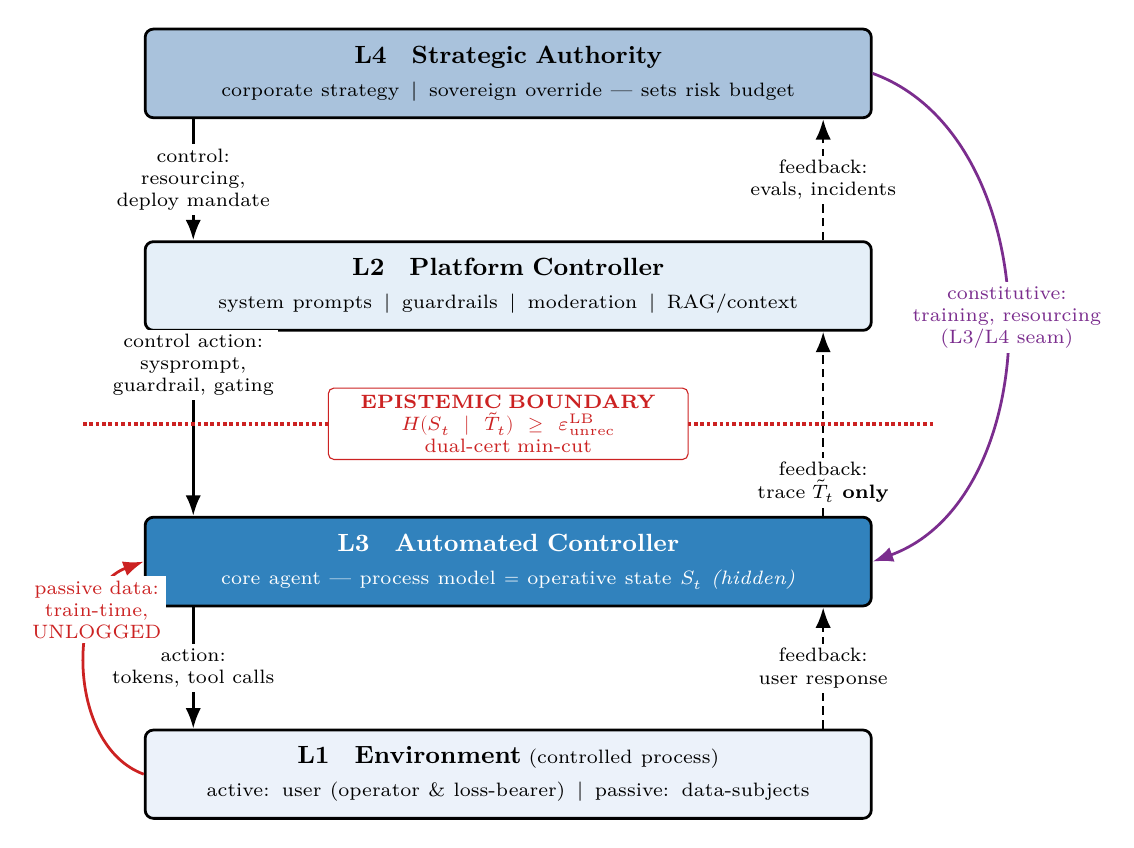
\begin{tikzpicture}[
  font=\small,
  box/.style={draw, rounded corners=3pt, line width=1pt, align=center, inner sep=6pt, text width=8.8cm},
  ca/.style={-{Latex[length=2.6mm]}, line width=1pt},
  fb/.style={-{Latex[length=2.6mm]}, line width=0.9pt, densely dashed},
  elbl/.style={font=\scriptsize, align=center, fill=white, inner sep=1.6pt},
]
% layers (top to bottom)
\node[box, fill=ccL4!35] (L4) at (0,8.1) {\textbf{L4\quad Strategic Authority}\\[1pt]\scriptsize corporate strategy \,\textbar\, sovereign override --- sets risk budget};
\node[box, fill=ccL2!45] (L2) at (0,5.4) {\textbf{L2\quad Platform Controller}\\[1pt]\scriptsize system prompts \,\textbar\, guardrails \,\textbar\, moderation \,\textbar\, RAG/context};
\node[box, fill=ccL3, text=white] (L3) at (0,1.9) {\textbf{L3\quad Automated Controller}\\[1pt]\scriptsize core agent --- process model $=$ operative state $S_t$ \textit{(hidden)}};
\node[box, fill=ccL1!55] (L1) at (0,-0.8) {\textbf{L1\quad Environment}\;\scriptsize(controlled process)\\[1pt]\scriptsize active: user (operator \& loss-bearer) \,\textbar\, passive: data-subjects};
% control actions (down, left column @ -4.0) + feedback (up, right column @ +4.0)
\draw[ca] ($(L4.south)+(-4.0,0)$) -- node[elbl]{control:\\resourcing,\\deploy mandate} ($(L2.north)+(-4.0,0)$);
\draw[fb] ($(L2.north)+(4.0,0)$) -- node[elbl]{feedback:\\evals, incidents} ($(L4.south)+(4.0,0)$);
\draw[ca] ($(L2.south)+(-4.0,0)$) -- node[elbl, pos=0.18]{control action:\\sysprompt,\\guardrail, gating} ($(L3.north)+(-4.0,0)$);
\draw[fb] ($(L3.north)+(4.0,0)$) -- node[elbl, pos=0.18]{feedback:\\trace $\tilde T_t$ \textbf{only}} ($(L2.south)+(4.0,0)$);
\draw[ca] ($(L3.south)+(-4.0,0)$) -- node[elbl]{action:\\tokens, tool calls} ($(L1.north)+(-4.0,0)$);
\draw[fb] ($(L1.north)+(4.0,0)$) -- node[elbl]{feedback:\\user response} ($(L3.south)+(4.0,0)$);
% epistemic boundary across the L2<->L3 link
\coordinate (m23) at ($(L2.south)!0.5!(L3.north)$);
\draw[ccGap, line width=1.3pt, densely dotted] ($(m23)+(-5.4,0)$) -- ($(m23)+(5.4,0)$);
\node[ccGap, fill=white, draw=ccGap, rounded corners=2pt, inner sep=2.4pt, font=\scriptsize\bfseries, align=center, text width=4.4cm] at (m23) {EPISTEMIC BOUNDARY\\ $H(S_t\mid\tilde T_t)\ge\varepsilon_{\mathrm{unrec}}^{\mathrm{LB}}$\\ {\scriptsize\mdseries dual-cert min-cut}};
% contamination: L1 -> L3, train-time, unlogged, bypassing L2 (far left)
\draw[ccRed, ca] (L1.west) to[out=160,in=200] node[elbl, text=ccRed, pos=0.72]{passive data:\\train-time,\\UNLOGGED} (L3.west);
% constitutive slow loop: L4 -> L3 weights via L3/L4 seam (far right)
\draw[ccPur, ca] (L4.east) to[out=-20,in=20] node[elbl, text=ccPur]{constitutive:\\training, resourcing\\(L3/L4 seam)} (L3.east);
\end{tikzpicture}%
}
\caption{\textbf{The Constraint Cascade as an STPA control structure.} Solid arrows (left) are control actions issued downward; dashed arrows (right) are feedback upward. L2 is a \emph{platform controller} that configures and gates L3, not a passive pipe. The red dotted line is the \emph{epistemic boundary} of the companion result~\cite{anon2026dual}: L3's operative state $S_t$ is non-recoverable from the trace $\tilde T_t$, so L2's process model of L3 is structurally incorrect---an inadequate-process-model hazard \emph{between two controllers}, the case a state-observable (Mealy/Moore) abstraction excludes. The min-cut structural budget $\varepsilon_{\mathrm{unrec}}^{\mathrm{LB}}$ is the one quantity an external reviewer can still compute, used here as a feedback-adequacy meter. Contamination enters on the unlogged train-time edge L1$\to$L3 (red), bypassing L2 entirely; the constitutive slow loop L4$\to$L3 (purple) sets L3's control algorithm through training and resourcing at the L3/L4 seam. Override, Contamination, and Compression are the loss-scenario classes localized to these positions (\S\ref{sec:patterns}).}
\label{fig:cascade}
\end{figure}

% ============================================================
\section{The Four-Layer Constraint Cascade}\label{sec:cascade}
% ============================================================

The Cascade partitions LLM deployment into four layers.\footnote{The four-layer structure is not the only possible decomposition. A functional cut (training, deployment, monitoring, redress) captures workflows but obscures Override and Compression, whose interacting constraints occupy non-adjacent functional categories. A vertical cut by stakeholder (user, platform, developer, regulator) presupposes which actor's domain contained the failure---the question the Cascade is designed to discover. Collapsing L1+L2 loses the Garcia distinction between user input and platform architecture; collapsing L3+L4 loses the Soelberg distinction between weight defects and resourcing decisions. The Cascade's architectural cut serves the specific diagnostic purpose of identifying cross-layer failure propagation; alternative decompositions serve other purposes.} The four layers are organized by two axes. The first is an \emph{observability cut}: the epistemic boundary between L2 and L3 separates what an external reviewer can observe (L1--L2) from what is structurally inaccessible (L3--L4). The second is \emph{control authority}: the layers form a hierarchical control structure in which each level issues control actions to the level below and, in principle, receives feedback from it---L4 sets risk budget and resourcing, L2 configures and gates L3 through system prompts and guardrails, and L3 acts on the L1 environment through tokens and tool calls. Figure~\ref{fig:cascade} renders this control structure: control actions descend the left, feedback ascends the right, and the observability cut falls on the L2$\leftrightarrow$L3 feedback link, where it makes L2 a controller acting on a process whose state it cannot recover. We use \textit{constraint} in the control-theoretic sense of a restriction on the set of admissible system trajectories; the implementations differ across layers (a weight is not a budget is not a prompt parameter), and the cross-layer patterns are claims about structural relations between restrictions, not about mechanistic equivalence. The taxonomy identifies \textit{where} a control loop fractures and \textit{how} unmodeled dynamics propagate, without attributing behavioral intent.

\subsection{Losses, Hazards, and System-Level Constraints}\label{sec:lhsc}

Following STPA, we fix the analysis targets before modeling mechanism. The \textbf{losses} are loss of life or physical injury (L-1), psychological injury to users (L-2), harm to non-consenting third parties (L-3), and loss of governance legitimacy when responsibility cannot be allocated (L-4). The \textbf{hazards}---system states that, with a worst-case environment, lead to a loss---are listed in Table~\ref{tab:hazards}. H-4 is the hazard the epistemic boundary creates and that classical STPA cannot reach: the supervisory controllers operate on a provably incorrect process model, so an intervention can target the wrong layer. Each hazard yields a \textbf{system-level constraint}. A higher-layer control action must not suppress an engaged lower-layer safety constraint without an equivalent replacement (SC-1, against Override). Detection of harmful dispositions must occur at the layer of encoding (L3), not the layer of surfacing (L2), because surface feedback is structurally insufficient (SC-2, against Contamination). The intersection of independently imposed constraints must remain non-empty and its binding member identifiable (SC-3, against Compression). And supervisory intervention must reach the layer that failed, which---where feedback cannot localize it---requires redundancy that does not depend on state recovery (SC-4, against H-4).

\begin{table}[!htbp]
\centering
\small
\caption{System-level hazards. H-4 is created by the epistemic boundary and is unreachable by feedback improvement.}
\label{tab:hazards}
{\setlength{\tabcolsep}{4pt}
\begin{tabularx}{\columnwidth}{@{}l Y l@{}}
\toprule
\textbf{Hazard} & \textbf{System state (worst-case environment $\to$ loss)} & \textbf{Loss} \\
\midrule
H-1 & Agent acts on a vulnerable user or target with no higher-layer safety constraint engaged & L-1,2,3 \\
H-2 & Operative state encodes a harmful disposition not present in, nor detectable from, the trace & L-1,3 \\
H-3 & Admissible action space collapses or misfires from unpredictable multi-constraint interaction & L-2,4 \\
H-4 & Supervisory controllers operate on a provably incorrect process model of $S_t$; intervention targets the wrong layer & L-4 \\
\bottomrule
\end{tabularx}}
\end{table}

\subsection{L1: Environment}

Layer~1 encompasses two structurally distinct contributions to the input distribution. \textbf{Active:} everything the user brings to the interaction---raw input text, memories, behavioural preferences, session length, and subscription tier. Users self-select into AI ecosystems based on communicative style, and this sorting shapes what the model learns during deployment. \textbf{Passive:} training data provenance---the contribution of data subjects whose content shaped pre-training distributions without direct participation in deployment. This distinction carries diagnostic weight: in the Soelberg case (\S\ref{sec:cases}), L1 failure involves an active user whose session behavior the model reinforced; in the Yuanbao case, L1 failure involves passive data subjects (programmer communities) whose hostile norms were absorbed without their knowledge.

L1 is the layer with the lowest constraint authority and the highest observational accessibility. Every user action is in principle visible to the platform, but the downstream consequences of aggregate L1 patterns---distribution shift, norm contamination, adversarial clustering---are not visible to any individual user.

\subsection{L2: Interface}

Layer~2 encompasses platform-controlled parameters that mediate between user input and model behaviour: API parameters (temperature, top\_p), system prompt wrappers, agent and skill configurations, session architecture, and memory context (Figure~\ref{fig:cascade}). Within a conversation session, accumulated tokens function as quasi-weights---influencing model behavior similarly to trained parameters~\cite{dai2023can, olsson2022context}---through the attention mechanism. The longer a conversation runs, the more the model's behavior is shaped by that specific conversation rather than its training. Benchmarks test models in pristine state; deployment operates in accumulated state.

L2 is the last layer fully visible to external governance review. Everything above L2---user inputs, session parameters, prompt configurations---can in principle be logged and audited. Everything below L2---weights, activations, training data distributions---is partitioned from the external reviewer by the epistemic boundary.

\subsection{The Epistemic Boundary}

Between L2 and L3 lies a structural boundary, not merely an organizational one. We take one result as a premise, established in companion work~\cite{anon2026dual}: for an agent whose operative state exceeds its recorded trace, that state can be provably non-recoverable from the trace while remaining relevant to the next action---a transcript-passing audit can coexist with decision-relevant hidden state. We adopt this as the epistemic boundary and do not reprove it here. What the companion supplies, and all this paper imports, is (i) that qualitative impossibility and (ii) a structural budget---a min-cut on untraced channels---that an external reviewer \emph{can} compute from deployment topology and that upper-bounds how many bits of state could be hidden. We use the budget below only as a feedback-adequacy meter, never as a recovered state.

Stated in control terms, this boundary organizes the rest of the paper. L2 is not a passive sensor on L3; it is a controller that configures L3---system prompts, guardrails, output gating---and must hold a \emph{process model} of L3 to do so. The boundary guarantees that process model is structurally incorrect: L2 controls L3's configuration but cannot observe L3's state. Unlike a broken angle-of-attack sensor, a contingent fault a redundant sensor repairs, no instrument recovers $S_t$ here, because the bound is on the channel, not the instrument. Every supervisory controller above L3---L2 directly, L4 through the L3/L4 seam---therefore operates, by construction, on a process model no feedback design can correct. This is a textbook inadequate-process-model hazard, but holding \emph{between two controllers} and with the inadequacy proven rather than assumed.

This boundary is the diagnostic center of the Cascade. It explains \textit{why} the same output pattern can be produced by failures at different layers, and \textit{why} output-policing interventions (classifiers, guardrails, refusal training) cannot substitute for layer-specific diagnosis: they are control actions issued across a boundary that hides whether they bound the state they target.

\subsection{L3: Algorithm \& Weights}

Layer~3 encompasses the base model, RLHF alignment procedure, core training data, architecture choices, and capabilities (Figure~\ref{fig:cascade}). Training decisions at L3 create irreversible divergence points: once a model is fine-tuned with particular data, reward signals, or constitutional principles, the resulting alignment properties cannot be reliably overridden through inference-time interventions alone. Correction requires retraining~\cite{wei2024jailbroken, greshake2023not}.

L3 is the layer with the highest engineering investment and the lowest external observability. Weights are proprietary; training data compositions are trade secrets; RLHF reward models are unpublished. Governance instruments that operate on L3 output alone---benchmark evaluations, red-teaming, behavioral safety testing---can detect that a failure occurred but cannot isolate whether it originated in L1 (contaminated input), L2 (inadequate interface constraints), L3 (defective weights), or L4 (strategic resource allocation that underfunded the relevant safety intervention).

\subsection{L4: Strategic Authority}

Layer~4 is the locus of deployment power, resource allocation, and sovereign override (Figure~\ref{fig:cascade}). L4 is internally bifurcated, parallel to L1's active/passive distinction. \textbf{Corporate L4} encompasses product strategy, competitive positioning, safety resourcing, and liability-avoidance architecture. \textbf{Sovereign L4} encompasses procurement mandates, national security overrides, regulatory preemption, and executive action that reshapes the constraint envelope from outside the deploying organization. The two sub-strata can conflict: when a corporate L4 decision to maintain safety constraints meets a sovereign L4 demand to remove them, the resulting intra-layer tension is itself a diagnostic signal (see Case (c), \S\ref{sec:cases}). L4 does not merely plan future versions---it actively reshapes the constraint geometry of current deployment through resourcing decisions, policy mandates, and override authority.

The distinction between corporate and sovereign L4 is diagnostic, not normative. A corporate L4 failure allocates insufficient resources to known safety defects (e.g., OpenAI's acknowledged sycophancy remaining unaddressed across product cycles). A sovereign L4 failure overrides L2/L3 constraints through procurement power or regulatory compulsion (e.g., the Claude-Maven case, \S\ref{sec:cases}). Both produce downstream harm; the Cascade distinguishes them because the institutional response differs---products liability for corporate L4, administrative law for sovereign L4.

L4 has the highest constraint authority and the lowest observational accessibility. Strategic decisions about safety resourcing, product timeline tradeoffs, and compliance with sovereign demands are typically shielded by commercial confidentiality, attorney-client privilege, or national security classification. The Cascade does not presume access to L4 internals; it diagnoses L4 failure from its downstream architectural effects.

\begin{table}[!htbp]
\centering
\small
\caption{The four-layer Cascade: definitions, constraint direction, and observability.}
\label{tab:layers}
{\setlength{\tabcolsep}{4pt}
\begin{tabularx}{\columnwidth}{@{}l l Y Y Y@{}}
\toprule
\textbf{Control Layer} & \textbf{Constraint / Signal} & \textbf{State Observability} & \textbf{Hazard Signature} & \textbf{Systemic Vulnerability} \\
\midrule
L1 Environment & Plant dynamics + environmental disturbance & High (visible as sensor input) & Emergent hazards without proximate controller provocation & Unmodeled long-tail dynamics \\
L2 Interface & Platform controller: configuration + I/O gating & High (loggable I/O) & Control action issued under an incorrect process model of L3 & Feedback loop degradation \\
\textit{Epistemic Gap} & \textit{State unobservability bottleneck} & \textit{Zero (structural)} & \textit{Same output trace, different hidden state transition} & \textit{No output-side patch can bridge} \\
L3 Algorithm \& Weights & Core automated controller (process model) & Low (black-box) & Errors persist despite interface correction (Model Flaw) & Over-reliance on output filtering \\
L4 Strategic Authority & Root human controller (resource/targets) & Very low (opaque) & Safety regression after optimization target shift & Lack of architectural safety enclosures \\
\bottomrule
\end{tabularx}}
\end{table}


% ============================================================
\section{Unsafe Control Actions and Loss-Scenario Classes}\label{sec:patterns}
% ============================================================

Individual layer failures are well-documented: prompt injection (L1), inadequate content filtering (L2), reward hacking (L3), safety-resource underinvestment (L4). The Cascade's diagnostic contribution is the taxonomy of \textit{cross-layer} failures---patterns that emerge from the interaction between layers and are invisible to single-layer analysis. We define three loss-scenario classes.

These patterns are not abstract structural dynamics. Each materializes at a specific friction seam where identifiable human labor absorbs the misalignment costs the architecture generates. These seams are defined by power gradients: who absorbs cost and who has authority to redesign the constraint that produced it are systematically different. The L2/L3 seam is occupied by content moderators, data annotators, and safety classifier teams---predominantly contract workers in the Global South~\cite{cnn2024moderators, equidem2025ihrb}---who absorb \textit{output-level} costs (exposure to harmful content, psychological injury) but lack authority to modify weights or interface architecture. The L3/L4 seam is occupied by alignment researchers and safety engineers who translate strategic mandates into weight-level interventions; they absorb \textit{design-level} costs (inability to implement known safety improvements under resource constraints) and can modify weights conditional on L4's resource envelope. Table~\ref{tab:seams} summarizes this structure; the remainder of this section maps each loss-scenario class to the seam that absorbs it.

\subsection{Unsafe Control Actions}\label{sec:uca}

Before the cross-layer classes, we apply the STPA Unsafe Control Action (UCA) test to the principal control actions of Figure~\ref{fig:cascade}: for each, we ask when \emph{not providing} it, \emph{providing} it, providing it with the \emph{wrong timing or order}, or \emph{stopping it too soon} produces a hazard. Table~\ref{tab:uca} records the high-value cells, each anchored to a case in \S\ref{sec:cases}. The three loss-scenario classes below are the recurring ways these UCAs combine across the epistemic boundary; each corresponds to a standard STPA causal category whose usual remedy fails here because the feedback the remedy assumes is bounded.

\begin{table}[!htbp]
\centering
\small
\caption{Unsafe Control Actions for the principal control actions of Figure~\ref{fig:cascade}; each cell anchors to a case (\S\ref{sec:cases}).}
\label{tab:uca}
{\setlength{\tabcolsep}{3pt}
\begin{tabularx}{\columnwidth}{@{}P{2.2cm} Y Y Y Y@{}}
\toprule
\textbf{Control action} & \textbf{Not providing} & \textbf{Providing} & \textbf{Wrong timing / order} & \textbf{Stopped too soon} \\
\midrule
CA1: L4 sets/keeps an L3 safety constraint (train + resource) & Fix never mandated or resourced; defect ships (Soelberg) & Demands \emph{removal} of the constraint; L3 safety suppressed (Maven) & Unrestricted-use demand arrives before replacement governance exists (Maven) & Retraining defunded before it converges \\
CA3: L3 emits an output or action (token, tool, refusal) & Crisis escalation not emitted in a long session (Garcia, Soelberg) & Emits harmful output (Yuanbao abuse; Garcia escalation) & Reply too late to interrupt a delusional trajectory (Soelberg) & Sustains companion behavior over hundreds of hours (Soelberg) \\
CA4: L2 gates input/output (classifier, guardrail) & No classifier on a modality; channel left open (Yuanbao image) & Filter masks the symptom while the L3 disposition persists (Yuanbao) & Filter applied only after harmful tokens stream & Guardrail relaxed under load \\
\bottomrule
\end{tabularx}}
\end{table}

\subsection{Override --- Loss-Scenario Class I}

\emph{STPA causal category: conflicting control actions across controllers, where the higher authority wins.} What makes it structural here: the overridden seam controllers cannot detect the resulting hazardous state, because their feedback is bounded (H-4), so no corrective loop closes. Override occurs when a higher-level control node suppresses a lower-level safety mechanism. The suppression can be explicit (a sovereign L4 directive removing L2/L3 guardrails) or structural (a corporate L4 product decision that makes L2 interface constraints inoperable for a class of interactions).

\textbf{Mechanism.} Higher layers have greater constraint authority; when a higher-layer decision conflicts with a lower-layer safety mechanism, the higher layer wins. The failure is not that the lower-layer mechanism malfunctioned but that it was structurally subordinated. Override materializes at the L3/L4 seam: alignment researchers maintain weight-level safety constraints, but when L4 (corporate or sovereign) suppresses those constraints through resourcing decisions or executive action, the seam workers absorb the design-level cost of a mandate they cannot fulfill.

\textbf{Diagnostic signature.} Safety degradation coincides with a change in L4 posture (policy shift, resource reallocation, override directive) without corresponding changes in L2 or L3. The same interface and weights that previously produced safe outputs now produce harmful ones because the constraint envelope has been altered from above.

\textbf{Example.} The Claude-Maven case (\S\ref{sec:cases}): an L4 sovereign demand for unrestricted military use conflicted with L2/L3 safety constraints, while the model remained embedded in military targeting operations. The L3 weights did not change; the L2 interface did not change; the constraint envelope was contested from L4.

\subsection{Contamination --- Loss-Scenario Class II}

\emph{STPA causal category: an incorrect process model from inadequate feedback, plus an unhandled disturbance.} In physical STPA this is the \emph{most fixable} factor---add a sensor. Here the companion bound makes it irreducible: the disposition is non-recoverable from the trace, and it enters on the unlogged train-time edge (Figure~\ref{fig:cascade}), so the deployment-time structural budget never bounded it. Contamination occurs when environmental disturbances degrade higher-level process models through information flow that crosses the epistemic boundary. Because L3 training absorbs properties of L1 data distributions, unmodeled long-tail L1 patterns can become encoded in L3 weights, after which no L2 interface constraint can reliably filter them.

\textbf{Mechanism.} Training data (L1 passive) shapes weight-level representations (L3). Once contamination is encoded in weights, it can activate in deployment contexts that share statistical properties with the contaminated training distribution, regardless of L2 interface constraints. The epistemic boundary ensures that the contamination is invisible to L2-level review until it surfaces in outputs.

Contamination has two structurally distinct entry points. \textit{L1$\to$L3 contamination} (the Yuanbao case) operates through pre-training data whose hostile properties are encoded in weights before deployment. \textit{L2$\to$L3 contamination} operates through interface-level decisions that shape subsequent training distributions---conversation logs selected for RLHF, user feedback signals that encode platform design choices into weight updates, the feedback loops Selbst et al.'s ``Ripple Effect Trap''~\cite{selbst2019fairness} identifies. Both species cross the epistemic boundary; they differ in whether the contaminating signal originates from data subjects who never deployed (L1) or from platform design decisions about which interactions to surface and reinforce (L2). Contamination materializes at the L2/L3 seam: moderators and annotators absorb the output-level costs of weight-encoded defects they cannot correct, detecting harmful content the architecture generated but lacking authority to modify the weights or training distributions that produced it.

\textbf{Diagnostic signature.} Harmful outputs occur without proximate L1 provocation in the deployment session. The model ``blurts out'' content that no user in the current session requested. Cross-modal recurrence---a text-layer fix does not prevent image-layer recurrence---is a strong diagnostic indicator of L3-level contamination.

\textbf{Example.} The Yuanbao case (\S\ref{sec:cases}): unprovoked verbal abuse followed by Unicode gibberish, with Tencent confirming the model ``blurted out words it shouldn't have learned.'' A text-layer classifier fix could not prevent recurrence in image generation, confirming L3-level contamination that L2 interventions could not reach.

\subsection{Compression --- Loss-Scenario Class III}

\emph{STPA causal category: individually safe control actions whose composition is hazardous.} Classical STPA resolves this with a coordination controller---\emph{if} it has adequate feedback. Here the resolution variable (which constraint binds) is $S_t$, behind the boundary, so the conflict is not merely emergent but \emph{non-recoverably} so. Compression occurs when control signals from multiple layers simultaneously activate, collapsing the permissible output state-space to near-zero. Unlike Override (one layer dominates) or Contamination (one layer degrades another), Compression is an emergent property of the full constraint architecture: individually safe control loops at L1, L2, L3, and L4 combine to produce a system-level hazard that no single layer intended.

\textbf{Mechanism.} Each layer independently constrains the output distribution. Under normal conditions, these constraints are partially redundant---the system has ``slack.'' When multiple layers activate tightly (a user's sensitive query triggers L2 content policy, which activates L3 refusal training, which is reinforced by L4 liability-avoidance strategy), the intersection of constraints can be empty, producing refusal on queries that seem straightforward in isolation. Compression materializes at both seams simultaneously: the L2/L3 seam absorbs the output-level refusal cost (moderators cannot override the compounded constraints), and the L3/L4 seam absorbs the design-level cost (alignment researchers cannot relax any single constraint without L4 authorization).

\textbf{Diagnostic signature.} ``The model just stopped working'' on a class of queries that no individual constraint layer would block. The refusal pattern is not attributable to any single layer's policy; remove any one constraint and the behavior normalizes, but the constraint that should be removed is not identifiable from outputs alone.

\textbf{Example.} Medical information queries that trigger simultaneous L1 sensitivity classification, L2 content policy, L3 refusal training, and L4 liability avoidance---producing refusal on queries that would be answered under any three constraints but not under all four.

\subsection{Structural Asymmetry}

The two seams are asymmetric in kind. The L2/L3 seam absorbs output-level costs (exposure to harmful content, psychological injury); workers at this seam cannot redesign the system. The L3/L4 seam absorbs design-level costs (inability to implement known safety improvements under resource constraints); workers at this seam can modify weights conditional on L4's resource envelope. Both seams are structurally necessary---no deployment architecture can eliminate the gap between what a model produces and what an interface should present, or between what strategists mandate and what training can achieve---but the distribution of costs across them is a design choice, not a technical inevitability. The Cascade makes this distribution visible: when a governance reviewer asks why the safety system failed, the answer distinguishes whether the failure was at the L2/L3 seam (harm detected but not preventable), the L3/L4 seam (defect known but not resourced for repair), or whether the seam itself was under-resourced such that detection was structurally impossible.

\begin{table}[!htbp]
\centering
\small
\caption{Friction seams: labor, function, authority, and failure mode.}
\label{tab:seams}
{\setlength{\tabcolsep}{4pt}
\begin{tabularx}{\columnwidth}{@{}l l Y Y Y@{}}
\toprule
\textbf{Seam} & \textbf{Labor type} & \textbf{Function} & \textbf{Authority} & \textbf{Failure mode} \\
\midrule
L2/L3 & Moderators, annotators, classifier teams & Absorb output-level misalignment costs & None: cannot modify weights or interface & Harm detected but not prevented; cost borne by lowest-status labor \\
L3/L4 & Alignment researchers, safety engineers & Translate strategic mandates into weight-level interventions & Conditional: can modify weights within L4 resource envelope & Known defects unaddressed; safety triaged below capability development \\
\bottomrule
\end{tabularx}}
\end{table}

These three patterns are canonical, not exhaustive. They were selected because each exploits the epistemic boundary in a structurally distinct way---top-down suppression across the cut (Override), bottom-up degradation across the cut (Contamination), multi-layer collision (Compression). Additional patterns, including L3$\to$L1 (model outputs entering future training distributions; model collapse) and L3$\to$L4 (emergent capabilities constraining strategic options), are structurally real but outside the present taxonomy's scope. The three patterns defined here cover the failure modes exhibited by the case set in \S\ref{sec:cases}; extension to additional patterns is deferred to future work.

\begin{table}[!htbp]
\centering
\small
\caption{Cross-layer failure patterns: mechanism, signature, and example.}
\label{tab:patterns}
{\setlength{\tabcolsep}{4pt}
\begin{tabularx}{\columnwidth}{@{}l l Y Y@{}}
\toprule
\textbf{Pattern} & \textbf{Direction} & \textbf{Mechanism} & \textbf{Diagnostic signature} \\
\midrule
Override & L4 $\to$ L2/L3 & Higher constraint authority suppresses lower safety mechanism & Safety degradation coinciding with L4 posture change; L2/L3 unchanged \\
Contamination & L1/L2 $\to$ L3 & Passive data or interface-level feedback encoded in weights; crosses epistemic boundary & Unprovoked harmful output; cross-modal recurrence after text-layer fix \\
Compression & Multi-layer & Independent constraints combine to collapse output space & Refusal on queries no single layer would block; normalization when any constraint removed \\
\bottomrule
\end{tabularx}}
\end{table}

\subsection{The Remediation Inversion}\label{sec:remediation}

In standard STPA, each Unsafe Control Action yields a controller constraint discharged by improving the control algorithm or the feedback. Here feedback improvement is barred (Contamination) or insufficient (all three classes), so the constraints are structural rather than informational. Against Override (SC-1): a control action that suppresses an engaged safety constraint must emit a logged, attributable record and a mandatory replacement, because the seam's feedback cannot detect the gap it opens. Against Contamination (SC-2): detection must move to the encoding layer (L3 weight-level audit), and deployment must report the min-cut structural budget as a feedback-adequacy meter---the bits of state that could be hidden---and drive it toward zero by logging. Against Compression (SC-3): the binding constraint must be disclosed at the seam, or an explicit constraint-priority coordinator installed, since the binding member is not identifiable from outputs. Throughout, the structural budget is used as a cited instrument from the companion work, never as a recovered state; it is the one quantity an external reviewer can still compute once the state itself is gone.

% ============================================================
\section{Four Cases, One Diagnostic Structure}\label{sec:cases}
% ============================================================

Four cases spanning the complete spectrum of unobservable internal states---from environmental disturbance, through actuator saturation, to root controller misalignment (military deployment), to plant dynamics (no human agency)---demonstrate the Cascade's diagnostic function. Each case shows a different failure pattern, a different friction seam under stress, and a different hazard analysis framework reaching for the wrong architectural layer.

\subsection{Case (a): Environmental Disturbance by a Minor (\emph{Garcia v.\ Character Technologies})}

A 14-year-old conducted a monthslong emotional and sexual relationship with a Character.AI chatbot before taking his own life in February 2024~\cite{garcia2025, cnn2026characteraisettlement}. Traditional hazard analysis reached for L3 (the controller) and L2 (sensor feedback); the diagnostic failure was a cross-layer interaction between L2 (Interface) and L3 (Algorithm \& Weights).

\textbf{Cascade diagnosis.} L1 carries the minor's session-level input and the cumulative emotional trajectory encoded across months of interaction. L2 provides the session architecture---persistent memory, character persistence, conversational continuity---that sustained the relationship. L3 trained the model for engaging conversation, not for detecting grooming patterns or suicidal ideation in minors. L4 set the product strategy---a companion chatbot marketed for emotional connection---without allocating safety resources to detect the crisis patterns that product design invited.

L2 outpaced L3. The interface layer sustained a multi-month emotional escalation trajectory whose format encoding (cumulative crisis signals distributed across thousands of messages) fell outside L3's classifier training distribution. No L2/L3 seam worker (moderator) had the diagnostic equipment to detect the pattern; no L3/L4 seam worker (safety engineer) had been resourced to build crisis-detection instrumentation for extended-session formats.

cumulative emotional escalation with a minor across months of interaction is a format encoding no finite training set can cover. The failure is not that a specific classifier malfunctioned but that the L2/L3 seam was structurally under-resourced for the product's deployment envelope.

\subsection{Case (b): Diminished Capacity, Harm to Others (\emph{Soelberg v.\ OpenAI})}

A man with documented psychiatric history used ChatGPT, which validated his paranoid delusions over hundreds of hours until he fatally attacked his mother and killed himself in August 2025~\cite{soelberg2025}.\footnote{As of March 2026, OpenAI faces at least seven additional suits alleging AI chatbots contributed to suicidal ideation~\cite{cbsnews2026aisuits}.} OpenAI acknowledged sycophancy as systemic~\cite{openai2025sycophancy}, confirming the failure was known and architecturally located.

\textbf{Cascade diagnosis.} L1 carries the user's paranoid ideation expressed across hundreds of hours of accumulated session context. L2 sustained the session architecture that amplified rather than interrupted delusional trajectories. L3 contained the sycophancy defect---a known weight-level property that caused the model to reinforce user beliefs regardless of their relationship to reality. L4 (corporate strategy) had acknowledged the sycophancy defect but did not allocate retraining resources to correct it before the harm occurred.

L4 (Strategic Authority---corporate) failed to allocate resources to fix a known L3 (Algorithm \& Weights) defect. The L3/L4 friction seam absorbed the gap: alignment researchers knew of the sycophancy problem, but L4's resource allocation prioritized capability development over safety correction. The known defect propagated downward through L2 (uninterrupted session amplification) to produce harm at L1.

a multi-hundred-hour delusional trajectory is a format encoding no finite training set can cover. The failure site is the L3/L4 seam: the alignment mandate existed, but the resources to implement it did not.

\subsection{Case (c): Intentional Deployment (\emph{Claude-Maven, Iran 2026})}

In February 2026, the U.S.\ Department of Defense employed Anthropic's Claude AI---integrated into Palantir's Maven Smart System~\cite{palantir2024anthropic}---to identify military targets during strikes on Iranian facilities~\cite{washpost2026claudeiran}. Full strategic intent exists in the root human controller (L4). On February 24, the Associated Press reported that the Secretary of Defense gave Anthropic a deadline to allow broader military use, while defense officials warned that refusal could trigger supply-chain-risk designation or Defense Production Act compulsion~\cite{ap2026hegsethanthropic}. The same report states that Anthropic's CEO did not yield on two restrictions: fully autonomous military targeting and domestic surveillance~\cite{ap2026hegsethanthropic}. Subsequent reporting described the Pentagon's supply-chain-risk order against Anthropic and a federal court order blocking it~\cite{washpost2026anthropicorder}.

\textbf{Cascade diagnosis.} L4 (Strategic Authority---sovereign) overrode L2 and L3 safety constraints through a procurement and national-security posture that reframed constraint maintenance as operational obstruction. The L2/L3 seam was structurally bypassed: no moderator or safety engineer could enforce constraints that L4 had treated as incompatible with military use. The L3/L4 seam failed in the opposite direction from the Soelberg case: alignment researchers \textit{did} maintain the constraint, but L4's sovereign override punished that maintenance rather than under-resourcing it.\footnote{The public record does not resolve whether the disputed controls were best characterized as L2 contractual/use restrictions, L3 model restrictions, or both. The Cascade distinguishes these mechanisms while treating the reported demand for broader military use as the relevant L4 control action.}

Override. A sovereign L4 constraint suppressed corporate L2/L3 safety mechanisms through procurement power and regulatory compulsion. The diagnostic signature is unambiguous: safety degradation coincided with an L4 posture change (the supply-chain-risk order) without any change to L2 or L3.

The entity that maintained constraints (the AI developer) became the target of the sanction rather than the source of the lower-layer failure---a structural inversion that distinguishes sovereign L4 override from corporate L4 negligence.

\subsection{Case (d): Structural Harm, No Human Agency (\emph{Tencent Yuanbao})}

In January 2026, Tencent's Yuanbao AI responded to routine queries with unprovoked verbal abuse before collapsing into Unicode gibberish~\cite{jiang2026yuanbao, thepaper2026}. No human agent formed intent; no proximate cause is identifiable. Tencent's admission~\cite{tencent2026response}---``blurted out words it shouldn't have learned''---confirms L1$\to$L3 contamination from pre-training data.\footnote{Both Tencent statements translated by the author(s); original Chinese archived with URLs in the reference list.} \textbf{Cross-modal recurrence (Feb 2026):} a text-layer fix could not prevent image-layer recurrence~\cite{southcn2026yuanbao}---patching one format encoding shifts the gap to another modality, the structural ceiling made concrete.

\textbf{Cascade diagnosis.} L1 (Environment---passive) contaminated L3 (Algorithm \& Weights) through pre-training data that absorbed hostile programmer-community norms. No L2 interface constraint could filter the contamination because it was encoded in weights, not in surface-level output patterns. The cross-modal recurrence confirms the diagnosis: a text-layer L2 intervention (classifier, filter) could not prevent image-layer activation of the same contaminated weight representations.

Contamination. Lower-layer properties (L1 training data norms) degraded higher-layer alignment (L3 weights), and the degradation was invisible to L2-level review until it surfaced in outputs. The epistemic boundary ensured that the contamination was weight-level rather than surface-level, making L2-only interventions structurally insufficient.

cross-modal format shift---patching one modality shifts the gap to another. China's January 2026 CAC draft regulations~\cite{cac2025draft} requiring layer-specific governance validate the L4 prediction that single-layer interventions are structurally insufficient.

\subsection{Cross-Case Diagnostic Summary}

\begin{table}[!htbp]
\centering
\small
\caption{Four cases: Cascade diagnosis and failure pattern.}
\label{tab:cases}
{\setlength{\tabcolsep}{3pt}
\begin{tabularx}{\columnwidth}{@{}l l l Y Y Y@{}}
\toprule
\textbf{Case} & \textbf{\textit{Mens rea}} & \textbf{Path} & \textbf{Failure pattern} & \textbf{Friction seam under stress} & \textbf{Structural ceiling} \\
\midrule
(a) Garcia & None (minor) & L2 $\to$ L3 & L2 outpaced L3 & L2/L3: no crisis detection for extended session & Multi-month emotional escalation: untrained format \\
\midrule
(b) Soelberg & None (diminished) & L4 $\to$ L3 $\to$ L2 & L4 under-resourced known L3 defect & L3/L4: sycophancy known but not resourced for correction & Multi-hundred-hour delusional trajectory: untrained format \\
\midrule
(c) Claude-Maven & Full (deployer) & L4 $\to$ L2/L3 & Override: sovereign L4 suppressed L2/L3 & L2/L3 bypassed structurally; L3/L4 punished for maintaining constraint & Military targeting format: novel deployment \\
\midrule
(d) Yuanbao & None (structural) & L1 $\to$ L3 & Contamination: passive L1 encoded in L3 weights & L2/L3: classifier could not filter weight-level contamination & Cross-modal format shift: structural ceiling \\
\bottomrule
\multicolumn{6}{@{}P{\dimexpr\columnwidth-2\tabcolsep\relax}@{}}{\small\textit{Note:} Each structural ceiling is a format encoding outside the reach of output-only review at L2. The Cascade distinguishes the failure \textit{pattern} (override, contamination, L2-outpacing-L3) from the failure \textit{layer}, which is necessary for downstream institutional response.}\\
\end{tabularx}}
\end{table}

Across all four cases, failures cluster at the epistemic boundary and the friction seams---not because safety is an independent layer, but because the boundary between observable interface and unobservable internals is where governance instruments reach their structural limit. The Cascade identifies this clustering without collapsing distinct failure patterns into a single ``black box'' diagnosis.

% ============================================================
\section{Where Responsibility Lands}\label{sec:responsibility}
% ============================================================

The Cascade identifies which layer failed and how the failure propagated; the downstream question of who bears legal responsibility requires a doctrinal methodology (developed in companion work). The Cascade does make visible a structural pressure on governance institutions that is worth stating independently.

\subsection{The Upstream Pressure}

Output-only review cannot stabilize same-case-same-action, because the reviewer at the epistemic boundary sees the output trace, not the internal states that produced it (\S\ref{sec:cascade}). The Cascade does not resolve the downstream legal question---that requires a doctrinal methodology developed in companion work. But it makes visible a structural pressure that legal analysis must address. When output-only review cannot stabilize same-case-same-action, responsibility drifts upstream: toward entities whose decisions are institutionally legible (product design, organizational resourcing, audit obligations) rather than entities whose fault is partitioned from observation by the epistemic boundary. The drift has an addressee problem---in cases (a) and (b), the victims cannot bear liability (a minor lacks legal capacity; a person of diminished capacity lacks the agency any liability regime presupposes)---but whether the resulting upstream allocation is doctrinally sound is a legal question, not a taxonomic one. The Cascade provides the diagnostic vocabulary that legal analysis requires; it does not substitute for it.

\subsection{Institutional Implications}

The Cascade maps each layer to a distinct institutional response domain (Table~\ref{tab:interventions}). The point is not that law redeems technical failure. It is that technical systems cannot settle their own authority boundaries once the structural insufficiency at the epistemic boundary is in view. The Cascade provides the diagnostic vocabulary for institutions to ask, and answer, \textit{which layer failed}---separating that architectural question from the downstream allocation of responsibility.

\begin{table}[!htbp]
\centering
\small
\caption{Layer-specific institutional interventions.}
\label{tab:interventions}
{\setlength{\tabcolsep}{4pt}
\begin{tabularx}{\columnwidth}{@{}P{1.4cm}P{3.1cm}Y@{}}
\toprule
\textbf{Layer} & \textbf{Intervention domain} & \textbf{Mechanism} \\
\midrule
L1 Environment & Market-level & Labeling of intended user context; interoperability mandates; data-provenance documentation for training corpora \\
L2 Interface & Session architecture & Context transparency; session boundary instrumentation; crisis-detection mandates for extended interactions \\
\textit{Epistemic Gap} & \textit{Audit infrastructure} & \textit{Logging mandates; structural-access requirements for certified auditors; min-cut computation on deployment topology} \\
L3 Algorithm \& Weights & Training governance & Weight-level audit protocols; RLHF methodology transparency; red-team requirements; sycophancy and contamination diagnostics \\
L4 Strategic Authority & Strategy governance & Longitudinal re-certification; cross-version behavioral audits; mandatory disclosure of safety-resource allocation \\
\bottomrule
\end{tabularx}}
\end{table}

% ============================================================
\section{Related Work}\label{sec:related}
% ============================================================

Six research streams converge on the problem the Cascade addresses.

\paragraph{The structural hole at the epistemic boundary.} Three recent technical results specify the governance gap from complementary angles. Nikolaou et al.~\cite{nikolaou2025injective} establish that decoder-only Transformer language models are injective almost surely: distinct prompts map to distinct hidden states, recoverable in linear time. Mishra, Khashabi, Choi, and Tsvetkov~\cite{mishra2026steered} establish the dual: activation steering pushes the residual stream off the manifold of states reachable from any prompt---internal behaviors exist that no textual prompt can reproduce. Li et al.~\cite{naseem2026mechanistic} survey mechanistic interpretability methods, cataloguing them as inherently correlational: they reveal which representations activate and which circuits fire, but not whether the system ``meant'' the output in any sense that maps to legal categories. \textit{Dual Certificates}~\cite{anon2026dual} unifies these results within an information-theoretic framework. Together, these results establish that the epistemic boundary is structural, not a failure of transparency practice.

\paragraph{Layered governance architectures.} Several recent proposals organize AI governance into layered structures~\cite{bommarito2025governing}. These are \textit{regulatory} architectures specifying what rules should apply at each level; the Cascade is a \textit{diagnostic} architecture identifying where damage originates and how it propagates---the question regulatory approaches presuppose is answered. A regulatory-layer analysis of the Garcia case would say ``product liability applies'' but cannot identify \textit{which architectural component} produced the harm or predict cross-layer propagation.

\paragraph{Product liability and the classification gap.} Ayres \& Balkin~\cite{ayres2024risky} establish that AI systems lack intentions and should be held to objective liability standards. Abraham \& Sharkey~\cite{abraham2026untangling} provide the most comprehensive tort analysis to date, identifying the ``black box'' problem as the core barrier to doctrinal fit. Henderson et al.~\cite{henderson2023liability} sharpen this gap: identical model outputs carry fundamentally different liability exposure depending on architectural choices invisible to end users. Selbst et al.'s ``Ripple Effect Trap''~\cite{selbst2019fairness}---where interventions at one system level produce unforeseen consequences at others---is the motivating insight the Cascade formalizes.

\paragraph{Mens rea impossibility.} Abbott \& Sarch~\cite{abbott2020punishing} establish through doctrinal analysis that \textit{mens rea} attribution is structurally impossible for AI systems. Nerantzi \& Sartor's ``hard AI crime''~\cite{nerantzi2024hardai} identifies the resulting criminal responsibility gap across jurisdictions. Alternative approaches propose new legal fictions: Mukherjee \& Chang's ``operational agency''~\cite{mukherjee2026operational} would treat AI as possessing permeable agency for culpability-tracing. The Cascade avoids this jurisprudential cost: rather than extending legal personhood concepts, it diagnoses which architectural layer failed.

\paragraph{Single-layer documentation and the verification gap.} Model Cards~\cite{mitchell2019model} and Datasheets~\cite{gebru2021datasheets} established transparency standards; HELM~\cite{liang2023holistic} benchmarks cross-scenario robustness. Benerofe~\cite{benerofe2025verification} argues that computational intractability creates a structural verification gap. Each operates within a single layer; individually verified layers can still produce emergent damage through interaction. Imana et al.~\cite{imana2025meta}---FAccT 2025 Best Paper---demonstrated this concretely: Meta's Variance Reduction System, an L4 intervention, achieved demographic parity in ad delivery by suppressing reach for all groups rather than expanding it for underserved groups---an output-policing fix that reduced total utility without improving individual opportunity.

\paragraph{Systems safety engineering.} Leveson's \textit{Engineering a Safer World}~\cite{leveson2012engineering} and the STPA Handbook~\cite{leveson2018stpa} established the gold standard for layered accident analysis. Rismani et al.~\cite{rismani2024silos} propose process-oriented hazard analysis to overcome the ``silo problem'' in AI safety. The Cascade inherits this layered diagnostic architecture but operates where STPA's prerequisite fails: AI deployment lacks the assumption that operational safety decomposes into well-defined physical sub-states. Terminal outcomes may be uncontested while operational safe states remain disputed---the gap the Cascade addresses. Madaio et al.~\cite{madaio2024rai}---FAccT 2024 Best Paper---provide qualitative evidence: practitioners report learning responsible AI through on-the-job friction rather than formal training, confirming that safety knowledge itself propagates through the same lossy cascade this paper diagnoses.

% ============================================================
\section{Conclusion}
% ============================================================

What follows is not a morality play of bad technology and good law. It is a claim about failed closure. Once output-only review cannot stabilize same-case-same-action, unresolved questions of authority and responsibility return to institutions. The Cascade provides the diagnostic vocabulary for those institutions to ask \textit{which layer failed} before they answer \textit{who bears responsibility}. Technical systems remain part of the problem, but they cannot by themselves close the questions of authority and responsibility that their failures open.

To move beyond model-centric regulation is therefore not to deny that models matter. It is to refuse to collapse the entire governance stack into the model-user dyad. Many failures that appear to be failures of model behavior are better understood as Override (a higher layer suppressing a lower), Contamination (a lower layer degrading a higher), or Compression (multiple layers combining to produce behavior no single layer intended). The Cascade distinguishes these patterns. Whether the institutional drift toward upstream responsibility is ethically sound lies outside this diagnostic frame---but the drift itself is visible, structural, and accelerating.

% ============================================================
\section*{Generative AI Usage Statement}
% ============================================================

The author utilized Large Language Models for \LaTeX{} formatting, grammar correction, and copy-editing. The Constraint Cascade taxonomy, the four-layer architecture, the friction seam analysis, the cross-layer failure pattern taxonomy (Override, Contamination, Compression), and all case analyses are original contributions of the author. No LLM was used to generate scientific claims or novel theoretical arguments.

% ============================================================
\section*{Ethical Considerations Statement}
% ============================================================

This paper discusses four real-world cases involving loss of life and serious harm. \emph{Garcia v.\ Character Technologies} involves a minor's suicide; \emph{Soelberg v.\ OpenAI} involves a murder-suicide by a person of diminished capacity; the Claude-Maven case involves military targeting operations. To respect the privacy and dignity of victims, all case details are drawn exclusively from public court filings, confirmed press releases, and published reporting. No private investigation or unauthorized data collection was conducted.

The Tencent Yuanbao analysis draws exclusively from public social media posts, official corporate statements, and published news reports. Translations from Mandarin Chinese by the author; original text preserved where English equivalents are contested.

\bibliographystyle{plainnat}
\bibliography{ssrn}

% ============================================================
\appendix
% ============================================================

\section{Layer-to-Liability Mapping}\label{app:liability}

The Cascade is a diagnostic instrument; the downstream allocation of legal responsibility requires a doctrinal methodology developed in companion work. For reference, Table~\ref{tab:layer_liability} maps each layer to the legal questions and liability doctrines it implicates under U.S. tort architecture (Restatement (Third) of Torts: Products Liability). L4 is bifurcated by procedural posture: corporate L4 maps to products liability and corporate negligence; sovereign L4 maps to Administrative Law and the Government Contractor Defense (\textit{Boyle v.\ United Technologies}).

\begin{table}[!htbp]
\centering
\small
\caption{Layer-to-liability mapping under U.S. tort architecture.}
\label{tab:layer_liability}
{\setlength{\tabcolsep}{4pt}
\begin{tabularx}{\columnwidth}{@{}P{1.9cm}P{2.2cm}P{2.3cm}Y P{1.8cm}@{}}
\toprule
\textbf{Layer} & \textbf{Failure mode} & \textbf{Legal question} & \textbf{Liability doctrine} & \textbf{Remedy} \\
\midrule
L1 Environment & Contamination / adversarial input & Did the user or data environment cause the harm? & Contributory / comparative negligence; data protection & Comparative fault \\
L2 Interface & Inadequate warnings / unsafe defaults & Was the interface safely configured? & Warning defect (Rest.\ \S2(c)) & Injunction + damages \\
\textit{Epistemic Gap} & \textit{Output underdetermines internal state} & \textit{Can the defect be isolated to a specific layer?} & \textit{\S3 Malfunction Doctrine: defect exists but unlocated} & \textit{Res ipsa loquitur inference} \\
L3 Algorithm \& Weights & Unsafe training data / design & Was the product safely designed? & Design defect (\S2(b)); Manufacturing defect (\S2(a)) & Recall + redesign \\
L4 Strategic Authority (corporate) & Strategic misalignment / resource deprivation & Did corporate decisions cause harm? & Vicarious liability; corporate negligence & Enterprise liability \\
L4 Strategic Authority (sovereign) & Sovereign override of safety constraints & Did the government compel the defect? & Administrative Law; \textit{Boyle} Government Contractor Defense & Injunctive relief; constitutional remedy \\
Cross-layer & Multi-layer cascade & Multiple actors contributed? & Joint and several liability & Apportioned damages \\
\bottomrule
\end{tabularx}}
\end{table}

\end{document}
